\documentclass[main.tex]{subfiles}

\begin{document}

\section{Introduction}

\subsection{Background}

Cancer is the second most prevailing cause of death in the world, behind cardiovascular diseases. It was reported 14 million new cases of various cancers worldwide in 2019 \cite{porcine_2021} and as life expectancy increase in the world, it is also expected for cancer rates to increase. There are several treatments for cancers, among them is \gls{rt}, a treatment developed in the early 1900s using x-rays to irradiate harmful tumours. It is an effective and non-invasive procedure, capable of removing and preventing the growth of tumours. The main challenge of \gls{rt} is delivering a lethal dose to the tumour without harming healthy tissue in the patient. Children are especially vulnerable to the long term side effects of radiation therapy because of their bodies are still growing and is not fully developed yet.

\begin{figure}[!ht]
    \centering
    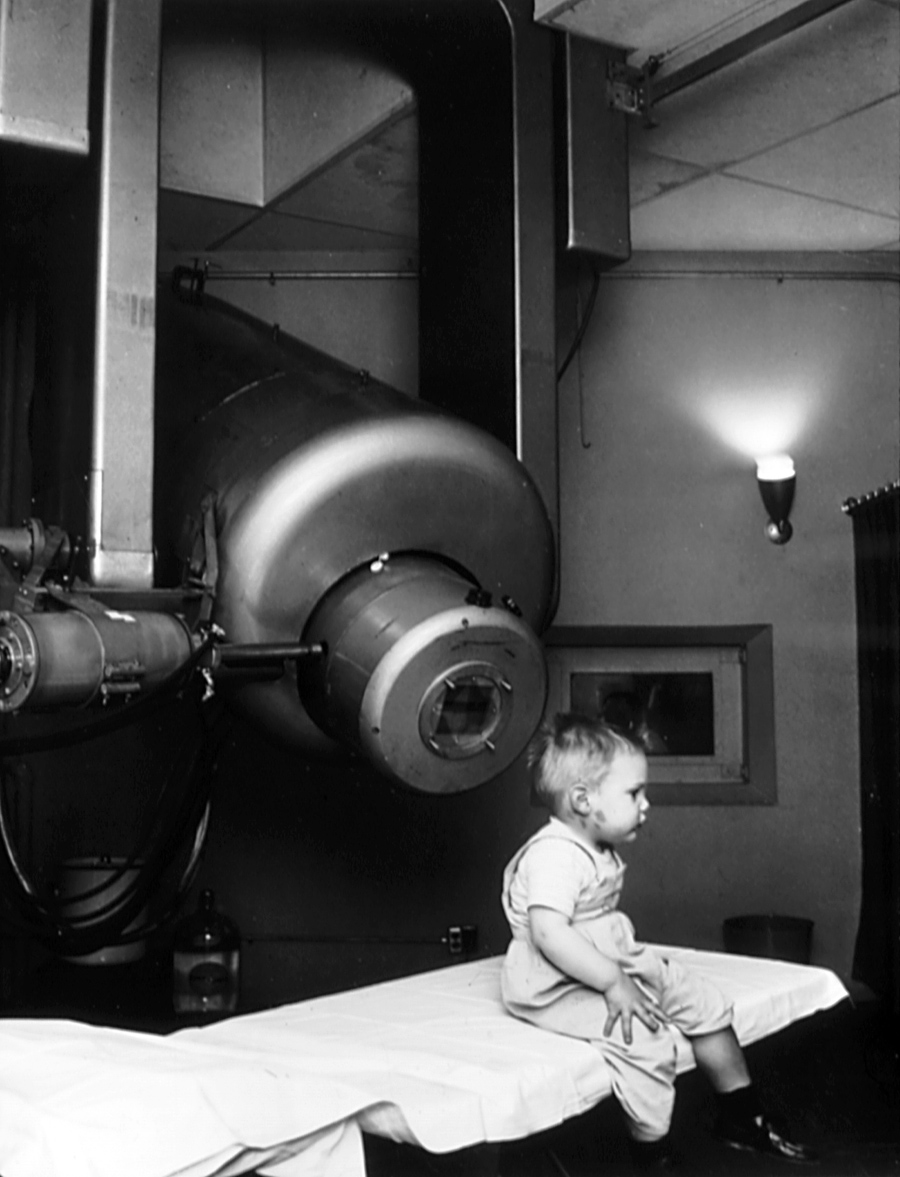
\includegraphics[scale = 0.4]{images/rt_intro.jpg}
    \caption{Image of the first pediatric patient being treated for retinoblastoma using radiotherapy.\cite{rt_intro}}
    \label{fig: rt_intro}
\end{figure}
\FloatBarrier


A \gls{ct}-scan is often done before radiation therapy as part of calculating the dose distribution. A \gls{ct}-scan is done by sending an x-ray source through the patient, and detectors behind the patient measures the energy of the exiting photons. The density of the tissue is proportional to the absorption of the X-ray beams, meaning photons going through bone structures will lose most of their energy, while photons going through soft or no tissue will retain most of the energy. This allows us to characterize the energy lost using the Hounsfield scale, a scale specifically designed for use in \gls{ct}-scans. With this, it is possible to create an image of the patients insides, which can be used for diagnostics, and can also be used to calculate the dose distribution. But even with these techniques, the patient will still receive a large radiation dose in nearby regions of the tumour. Using \gls{rt} in high-risk areas, such as the brain or heart can therefore lead to severe damage to the organs.  \par

Particle therapy is a new treatment that started developing in the mid 1900s as an alternative to \gls{rt}. Particle therapy was sought as an alternative because particles allows for  concentrating the dose distribution, which avoids damaging healthy tissue. Particles release very little of their energy while moving through a medium, it is not until the particle completely stops it effectively releases all its energy. This phenomenon is known as "Bremsstrahlung" and it allows us to deliver high doses of energy to a concentrated area while having relatively little entry dose and effectively zero exit dose. The moment when the particle releases all its energy is known as the "Bragg-Peak" and we can calibrate this "peak", targeting only the tumour inside the body. Knowing the \gls{rsp} of the medium the particles are sent through is essential to control the Bragg-Peak. A traditional \gls{ct}-scanner can be used to calculate the \gls{rsp}, this is done by measuring Hounsfield-units, and the convert Hounsfield units into \gls{rsp}. This conversion is not perfect and it will lead to higher uncertainty in the measurements of the \gls{rsp}. The stochastic nature of particles' energy loss also leads to higher uncertainties which makes it even more crucial to have precise measurements when performing particle treatment. Directly measuring the \gls{rsp} with a particle \gls{ct}-scan can circumvent the uncertainty stemming from converting from Hounsfield units. This has led to further research and development of particle based \gls{ct}-scan machines.



\subsection{Bergen PCT project}
Today the most common type of particle therapy is proton therapy; there are currently over 33 proton therapy centers in Europe. Norway plans to open two proton therapy centers by the end of 2024, one in Oslo and one in Bergen. The Bergen pCT-project is a collaboration with the University of Bergen, several other universities and companies to build a \gls{pct}-scanner to be used in particle therapy. The \gls{pct}-scanner is realized with a \gls{dtc} to measure the energy levels and trajectory of the protons exiting a patient exposed to a proton beam.

\begin{figure}[!ht]
    \centering
    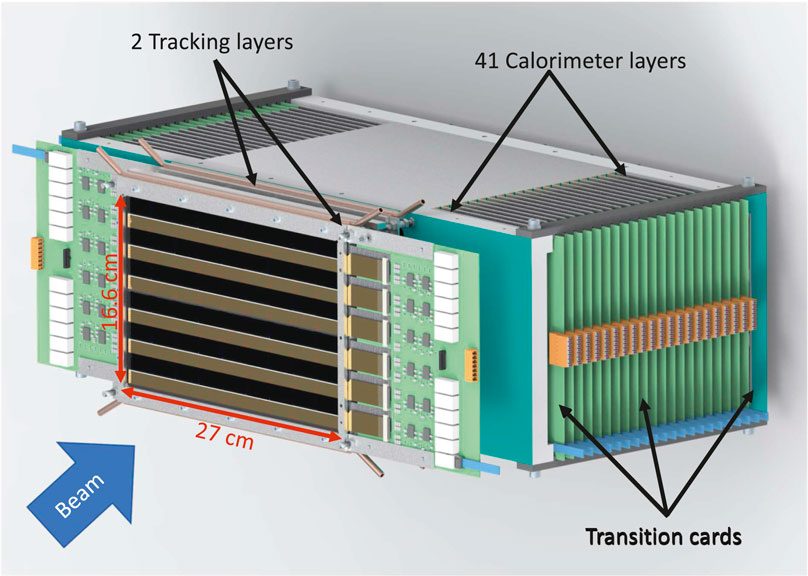
\includegraphics[scale = 0.5]{images/dtc.jpg}
    \caption{Image of the DTC to be used in the Bergen pCT project.}
    \label{fig: rt_intro}
\end{figure}
\FloatBarrier

The \gls{dtc} is developed using \gls{alpide}-chips that was originally used for the \gls{its} in the \acrshort{alice} experiment at \acrshort{cern}. The \gls{dtc} is made out of 43 layers, and a layer is made out of 12 strings with 9 \gls{alpide}-chips each. the protons enter the front of the detector and their energy is measured by the chips as they travel through each layer. 2 of the 43 layers is designated tracking layers, calculating the angle the protons exit the patient from. It is necessary to track the angle of the protons due to effects such as coulomb-scattering which can affect both the energy and trajectory of the protons. A \gls{dtc} is traditionally made with two tracking layers in the front and two layers in the rear of the \gls{dtc}, but the \gls{pct}-project only has the rear trackers. Such a \textit{single-sided} system has advantages over a \textit{double-sided} system, such as reducing cost and complexity of the system. A simplified block diagram of the \\gls{pct} system is shown in \autoref{fig: dcs_renewed}.

\begin{figure}[!htpb]
    \centering
    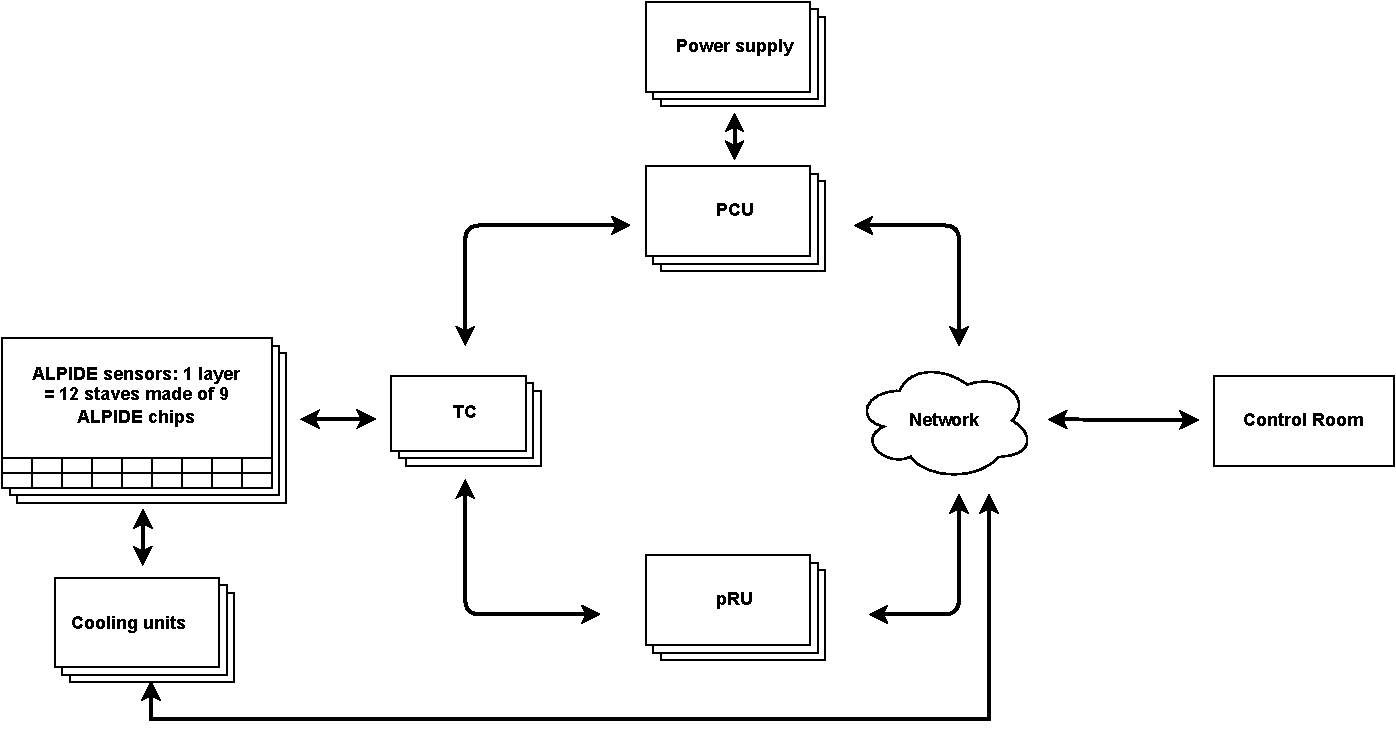
\includegraphics[scale = 0.65]{images/dcs_concept_renewed.pdf}
    \caption{Simplified block diagram of the pCT system.}
    \label{fig: dcs_renewed}
\end{figure}
\FloatBarrier

The figure shows the three different systems encompassing the \gls{alpide} sensors, power delivery, readout, and cooling, all being managed by the Control Room. The \gls{pcu} and \gls{pru} transfer power and perform readout of the strings, respectively, through the \gls{tc}s. Cooling is located next to the detector layers and is connected directly to the Control Room. All three systems are still in development, but the focus of this thesis will be on the power delivery system.

A separate \gls{mb} is responsible for delivering the power to the \gls{tc} and monitor temperature and current of the strings. Data transmission between the client and hardware is performed using IPbus, an established ethernet-based communication protocol often used in particle physics experiment. The \gls{mb} must be able to deliver enough current, and monitor temperature and current draw of the strings of \gls{alpide}-chips. The current plan is to have a power supply for each layer of the \gls{dtc} and a monitor board for each layer delivering the power to the \gls{tc}, while monitoring the strings. \par

The \gls{mb} uses a microcontroller to directly monitor the temperature and current draw of the layer, this allows us to quickly turn off strings if temperature or current exceeds safe ranges. For this purpose, the microcontroller has several configurable registers for threshold values and readings of analog current, digital current and temperature. The \gls{mb} requires a configuration system for powering the strings in a safe manner without damaging the equipment. A client-side monitoring system is also needed that is able to give the user accurate information of the strings during a run. A monitoring system is essential for troubleshooting and debugging. The configuration and monitoring systems must also be able to quickly and reliably receive and transmit data between the user and the monitor boards as slow configuration time could have a big impact in the usability of the instrument.

\subsection{Power Control and Monitoring}

The power delivery system requires both a configuration and monitoring system. The \gls{mb} uses a microcontroller that directly monitors and controls the power delivery to the strings which is useful to handle time critical events. If the current consumption or temperature of the strings reaches a critical level, then they are turned off as fast as possible by the microcontroller. There is also a need for a control and monitoring system that interfaces with the \gls{mb} itself. The microcontroller must be configured through some process and the user of the system needs a way to monitor the performance of the strings. It is common in the industry to use a standard for designing control systems called SCADA, so it is worthwhile to design our control system using those standards to ensure the system is standardized and well structured.

The configuration system must be able to configure the microcontroller with threshold values for current, voltage and temperature. Additionally, the system needs an algorithm for powering on the strings one-by-one. Turning on all strings simultaneously will cause a large power spike, which can damage the equipment. The configuration system does not have specific time constraint to it, since the microcontroller takes care of time critical events, however, the system should still not be too slow. The system should not be "laggy" for the user, meaning the computer should not lag when running the program, which is cumbersome for the user. Additionally, if the configuration process is slow, then repeated troubleshooting becomes a tedious process, which should be avoided. Therefore the configuration should ideally only take maximum 1-2 seconds to complete.

The monitoring system has similar requirements, it has no specific time constraint, but ideally it should still be quick and not feel "laggy" to the user. The monitoring also has a polling frequency, which determines how often it polls data from the microcontroller. To get good sampling of the parameters of the power delivery, the monitoring system should have a sampling frequency of minimum 1Hz, but ideally should be about 2-4Hz.

\subsection{Objective of this thesis}

The objective of this thesis is to design and build the configuration and monitoring system for the \gls{pct} power delivery to the detector layers. Many aspects of the systems must be assessed and considered to ensure they are suitable for the \gls{pct}-project. Both systems must be able to communicate with the microcontroller on the monitoring board and as such, an \acrshort{fpga}-solution is used with IPbus to receive and transmit data between client software and the microcontrollers. \autoref{fig: pcs_basic} shows a block diagram of the power delivery system.

\begin{figure}[!htpb]
    \centering
    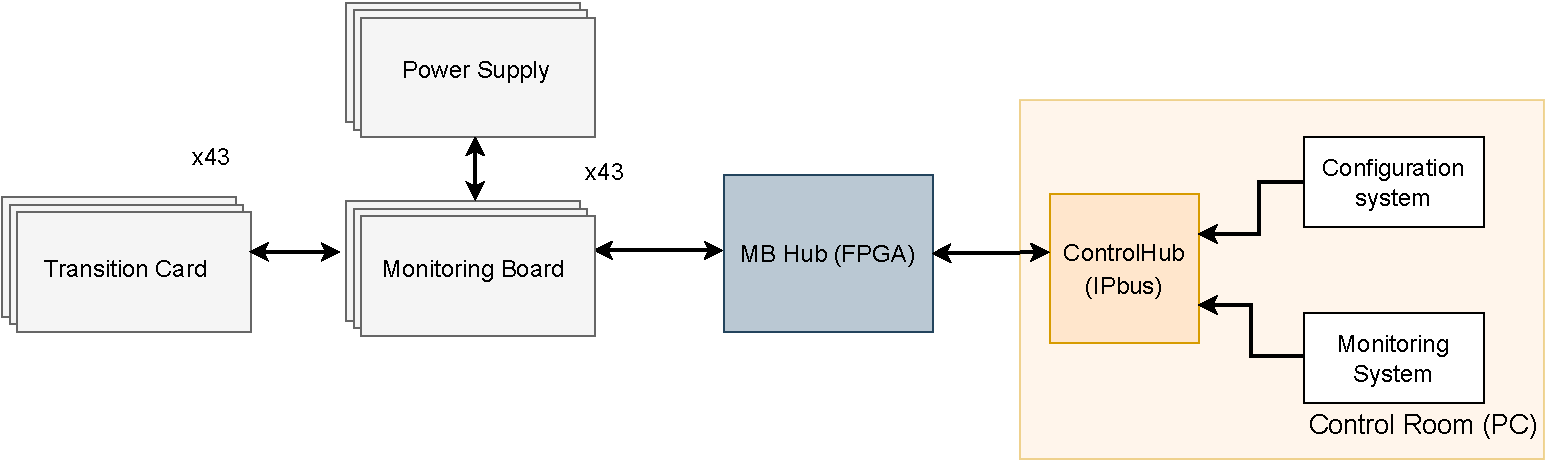
\includegraphics[scale = 0.65]{images/PCS basic overview.pdf}
    \caption{Block diagram of the power delivery system.}
    \label{fig: pcs_basic}
\end{figure}
\FloatBarrier

The work will focus on creating the configuration and monitoring systems that will interface with the \gls{mb}s and the MB Hub. This involves creating an \gls{api} for the \gls{mb}s, a \gls{hmi} and databases for storing the data.

The work performed will use a variety of software tools for communicating with IPbus and creating GUIs. The focus will be on creating a control system that is structured in a logical manner and is modular and generic. This will make the system easy to modify and expand upon, as well as troubleshooting, which is essential when working with a large control system. The cooling and readout systems does not have a complete control system in place, but if the power control system is generic, then parts of that system can be reused for cooling and readout as well. This would be to the benefit of the \gls{pct}-project, because it would be a lot simpler to manage three similar systems, than three isolated, custom systems.


The requirements for this control system is as follows:

\begin{itemize}
    \item Configure all relevant registers in the microcontrollers on the \gls{mb} for every layer.
    \item Store configuration data in a database allowing for easy loading and saving configuration sets.
    \item A GUI that allows a user with little knowledge of the system to load configuration sets.
    \item A powering-on algorithm that turns on the strings one-by-one, leading to a slow ramp-up of power usage, to avoid creating a large power spike.
    \item Periodically read current draw and temperature from each layer and store the data in a time series database.
    \item Display the monitoring data from each layer in intuitive and easy to understand graphs.
    \item A low and high level API to communicate with the IPbus module on the \acrshort{fpga} and the microcontroller on the \gls{mb}.
    \item Generic, modular \acrshort{oop} code that is easy to change and modify, so the system can be expanded upon and reused for similar projects in the future.
    \item The configuration process must not be "laggy" for the user and should not take more than a few seconds to complete.
    \item The The polling frequency of the monitoring process must at minimum be at 1Hz but ideally it should be at 2-4 Hz.
    \item The software design must follow software process standards and the control system standards laid out by SCADA.
    
The power system requires a low level API that can perform basic communication with \gls{mb}, and this \gls{api} becomes the base interface for the other \gls{api}s for monitoring and configuration. 

Following software process standards ensures that the system is structured in a logical manner, which helps the system being modular and generic. This means the system can be easily modified and expanded upon in future, which is a must for a control system with a long shelf time. Additionally, following the model for designing SCADA systems serves as a guideline for creating a structured and well documented control system.
    
    
\end{itemize}


\subsection{Structure of this thesis}

\textbf{Chapter 2 - Radiotherapy and Proton Therapy} \textit{This chapter goes through the theory of radiation and particle therapy, and also discusses the challenges with those treatments. The focus will be on how particle therapy can improve cancer treatment from traditional radiotherapy, and what must be considered when using particle therapy.} 

\textbf{Chapter 3 - PCT project} \textit{This chapter introduces the \gls{pct}-project, the background of the project, and gives an overview of the different components and systems that comprises the \gls{pct}-project. It will discuss the calorimeter and the design of the detector layers. Description of the control system for power delivery and readout is given, and general theory of control system development is discussed, with focus on SCADA systems.}

\textbf{Chapter 4 - PCS} \textit{This chapter will cover the power control system of the \gls{pct}-project. It will discuss the current design of the PCS and describe the various parts comprising it. The chapter will discuss the design of the control software, the FPGA hub, and the monitor board  of the PCS. The chapter will additionally cover the IPbus protocol, its characteristics and how it will be implemented in the control software.}

\textbf{Chapter 5 - Configuration System} \textit{This chapter will cover the design of the configuration system used in the power delivery system. It starts by going through the design of the configuration API and the layers of abstraction used in the lower level API for the PCS. It will then cover the design requirements of the configuration system, such as the powering algorithm, the setup of the database, and the GUI that will interface with the entire system. It will also discuss the theoretical configuration timing of the system, along with the measured timing performed on the prototype setup.}

\textbf{Chapter 6 - Monitoring System} \textit{The chapter will go over the design of the monitoring system for the power delivery system. The monitoring API is covered, describing the hierarchy of API classes and their functions. The chapter will then cover the monitoring database and the various features and web interfaces that is used to display data in the monitoring system. It then describes the characteristics of the monitoring operation, such as polling speed and storage space, and ends with discussing how one can optimize the data acquisition through data filtering and batching data points.}

\textbf{Chapter 7 - Testing and Verification} \textit{The prototype setup of the PCS is introduced and various tests is described for testing the entire PCS chain. The results of those tests is discussed and what they mean for the viability of the test setup. It will also go over simulation classes that was created to test API functionality with IPbus on software.}

\textbf{Chapter 8 - Discussion} \textit{This chapter discusses the work done in this thesis, what is still not complete or missing, and discusses how the work done for the power control system can be applied and reused for the other the cooling and readout systems in the \gls{pct}-project.}

\textbf{Chapter 9 - Conclusion} \textit{This chapter sums up the work done in this thesis and describes the future work that must be performed to make the system operational.}






\end{document}